\documentclass[12pt,a4paper,oneside, openany]{book}


\usepackage{lmodern}
\usepackage[table]{xcolor}
\usepackage{xcolor}
\definecolor{vert1}{rgb}{0.0,0.3.9,0.0}
\definecolor{bleu}{rgb}{0,0,0.5}
\definecolor{bleu3}{rgb}{1,0.2,0.2}
\definecolor{grisgris}{gray}{0.4}
\definecolor{grisclair}{HTML}{E7E7E7}
\definecolor{grisfonce}{HTML}{A5A5A5}
\definecolor{rougeUPS}{rgb}{0.6, 0.3, 0.3}

\fboxsep =0pt \parindent =0pt\parskip =12pt



\usepackage[utf8]{inputenc}
\usepackage[T1]{fontenc}
\usepackage[francais]{babel}
\usepackage[top=1.7cm, bottom=1.7cm, left=1.7cm, right=1.7cm]{geometry}
\usepackage{verbatim}
\usepackage[urlbordercolor={1 1 1}, linkbordercolor={1 1 1}, linkcolor=vert1, urlcolor=bleu, colorlinks=true]{hyperref}
\usepackage{tikz} %Vectoriel
\usepackage{listings}
\usepackage{fancyhdr}
\usepackage{multido}
\usepackage{amssymb}
\usepackage{eurosym}
\usepackage{array}
\usepackage{float}
\usepackage{graphicx}
\usepackage{pdfpages}

\newcommand{\US}{User Story}
\newcommand{\USs}{User Stories}

\newcommand{\story}[1]{ User story ``\textit{#1}'' }

\newcommand{\footnotesouvenir}[2]{
	\footnote{#2}
	\newcounter{#1}
	\setcounter{#1}{\value{footnote}}
}
\newcommand{\footnoterappel}[1]{
	\footnotemark[\value{#1}]
}

\newcommand{\remarque}[1]{
	\begin{center}
	\medskip
	\colorbox{remarque}{
		\begin{minipage}{0.85\textwidth}\medskip
\includegraphics[height=10px]{images/remarque.png} #1 \medskip\end{minipage}
	}
	\medskip
	\end{center}
}

\newcounter{exemples}

\newenvironment{exemple}[1]{
   \vspace{-2mm}

\refstepcounter{exemples}
   \begin{center}
	\medskip
      \begin{minipage}{0.9\linewidth}
}{%
~
      \end{minipage}
   \end{center}~
   \vspace{-2mm}
}%

\newcommand{\captionExemple}[1]{
	\begin{center}{\bsc{Exemple} \thechapter.\arabic{exemples}~--~}#1\end{center}
}


\DeclareTextFontCommand{\policeGlossaire}{\fontfamily{lmss}\selectfont}
\DeclareTextFontCommand{\policePackage}{\fontfamily{phv}\selectfont}
\DeclareTextFontCommand{\policeTitre}{\fontfamily{ptm}\selectfont}
\newcommand{\policeCode}[1]{\texttt{#1}}

\newcommand{\sectionfont}{%
	\fontencoding{\encodingdefault}%
	\fontfamily{pag}%
	\fontseries{bc}%
	\fontshape{n}%
	\selectfont
}

% numéro du chapitre
\DeclareFixedFont{\chapnumfont}{T1}{phv}{b}{n}{80pt}
% pour le mot « Chapitre »
\DeclareFixedFont{\chapchapfont}{T1}{phv}{b}{n}{16pt}
% pour le titre
\DeclareFixedFont{\chaptitfont}{T1}{phv}{b}{n}{24.88pt}


\usepackage{ifthen}

\newsavebox{\fmbox}
\newenvironment{fmpage}[1]
     {\begin{lrbox}{\fmbox}\begin{minipage}{#1}}
	  {\end{minipage}\end{lrbox}\fbox{\usebox{\fmbox}}}


\makeatletter

\title{Projet Agile --- \bsc{SCRUM}}

\def\top#1{\def\@top{#1}}

\def\sousTitre#1{\def\@sousTitre{#1}}
\sousTitre{Rubidium}

\def\location#1{\def\@location{#1}}
\location{Toulouse}

\date{\today}

%% Entete (Université..)  
\def\clap#1{
	\hbox to 0pt{\hss #1\hss}
}%
\def\ligne#1{%
	\hbox to \hsize{%
		\vbox{\centering #1}
	}
}%

% définition du haut de la couverture %
\def\haut#1#2#3{%
	\hbox to \hsize{%
		\rlap{
			\vtop{\raggedright #1}
		}%
		\hss
		\clap{	
			\vtop{\centering #2}
		}%
		\hss
		\llap{
			\vtop{\raggedleft #3}
		}
	}
}%

% Définition du bas de la couverture %
\def\bas#1#2#3{%
	\hbox to \hsize{%
	\hss \clap{\vbox{
	\centering \hspace{1.7cm}\newline
		\newline \newline \newline	\newline \newline \newline	\newline \newline \newline	\newline \newline \newline	\newline \newline \newline	\newline \newline \newline\newline #2 }
		}%
		\hss
	}
}%

% Zou, on peut construire la page de garde 
\def\maketitle{%
	\thispagestyle{empty}\vbox to \vsize{%
		\vspace{-25px}
		\vspace{5px}
		\haut{}{\@top}{}
		\vfill
		\begin{flushleft}
			David \bsc{Bernard}\\
			Mathias \bsc{Faure}\\
			Antoine \bsc{Incorvaia}\\
			Lucas \bsc{Le gouic}\\
			Antoine de \bsc{Roquemaurel}\\
			Clément \bsc{Vannier}\\
		\end{flushleft}

		\begin{flushright}
			\vspace{-3cm}
			\begin{tabular}{r@{~}l}
				Pour M. \bsc{Fernandez} 
			\end{tabular}
		\end{flushright}
		\vfill
		\vspace{1cm}
		\begin{flushleft}
			\policeTitre{\huge \@title}
		\end{flushleft}

		\par
		\hrule height 4pt
		\par

		\begin{flushright}
			\policeTitre{\Large \@sousTitre}
			\par
		\end{flushright}
		\vspace{3.2cm}
		\bas{}{ \@location, le \@date}{}
		\vspace{5px}
		\vspace{-15px}
	}%
	\cleardoublepage
}

\makeatother

\top{%
	Université Paul Sabatier -- Toulouse III\\
	IUT A - Toulouse Rangueil\\
	%\textbf{Projet tuteuré \#20}\\[1em]
}%

\makeatletter

\makeatother
\pagestyle{fancy}

\makeatletter
\def\thickhrulefill{\leavevmode \leaders \hrule height 1ex \hfill \kern \z@}
%% \chapter
\def\@makechapterhead#1{%
  \reset@font
  \parindent \z@
  \vspace*{10\p@}%
  \hbox{%
    \vbox{%
      \advance\hsize by -2cm
      \hrule height 0.4pt depth 0pt width \hsize
      \par
      \vskip 6pt%
      \hspace{20pt}%
      \parbox{420pt}{%
        \LARGE \bfseries #1
		}%
      \par
      \vskip 6pt%
      \hspace{20pt}%
      \hrule height 0.4pt depth 0pt width \hsize
	  \vspace{-30pt}
      }%
    \vbox{%
      \hsize=1.5cm%
      \begin{tabular}{c}
        \scshape \large \strut \@chapapp{} \\
        \colorbox{black}{\vbox{\hbox{\vbox to 1mm{}}\hbox{
			\color{white} \LARGE \bfseries \hspace{1mm}\thechapter\hspace{1mm}
		}\hbox{\vbox to 2cm{}}}}%
      \end{tabular}%
      }%
    }%
  \vskip 20\p@
}
%% \chapter*
\def\@makeschapterhead#1{%
  \reset@font
  \parindent \z@
  \vspace*{10\p@}%
  \hbox{%
    \vbox{%
      \advance\hsize by -0cm
      \hrule height 0.4pt depth 0pt width \hsize
      \par
      \vskip 6pt%
      \hspace{20pt}%
      \parbox{420pt}{%
        \LARGE \bfseries #1
		}%
      \par
      \vskip 6pt%
      \hspace{20pt}%
      \hrule height 0.4pt depth 0pt width \hsize
      }%
    }%
  \vskip 20\p@

}

\newlength{\sectiontitleindent}
\newlength{\subsectiontitleindent}
\newlength{\subsubsectiontitleindent}
\setlength{\sectiontitleindent}{-1cm}
\setlength{\subsectiontitleindent}{-.5cm}
\setlength{\subsubsectiontitleindent}{-.25cm}

\renewcommand{\section}{%
	\@startsection%
	{section}%
	{1}%
	{\sectiontitleindent}%
	{-3.5ex plus -1ex minus -.2ex}%
	{2.3ex plus.2ex}%
	{\sectionfont\Large}
}
\renewcommand{\subsection}{%
	\@startsection%
	{subsection}%
	{2}%
	{\subsectiontitleindent}%
	{-3.5ex plus -1ex minus -.2ex}%
	{2.3ex plus.2ex}%
	{\sectionfont\large}
}

\renewcommand{\subsubsection}{%
	\@startsection%
	{subsubsection}%
	{3}%
	{\subsubsectiontitleindent}%
	{-3.5ex plus -1ex minus -.2ex}%
	{2.3ex plus.2ex}%
	{\sectionfont\normalsize}
}

\makeatother



\lhead{Projet Agile --- \bsc{Scrum}}
\cfoot{\thepage}





\includeonly{
includes/avantPropos,
includes/sprint0, 
includes/sprint1, 
%includes/sprint2,
%includes/sprint3,
includes/annexes/tachesRedmine
}

\begin{document}
	\setcounter{tocdepth}{1}
	\setcounter{secnumdepth}{3}
	\maketitle
	\frontmatter
	\section*{Avant-propos}
\addcontentsline{toc}{chapter}{Avant-propos}
L'enseignement Agile a été mis en oeuvre à travers la création d'une application de gestion de 
surveillance d'examens, ce logiciel fut baptisé ``\textit{Rubidium}''.

Ce logiciel doit permettre aux enseignants de s'auto-affecter à la surveillance de partiels\footnote{
En effet, ils ont un quota d'heure de surveillance à respecter, ce logiciel permettra de les aider à savoir où ils en sont dans ce quota}, aux responsables de matières de créer et d'éditer des partiels et aux administrateurs de gérer en intégralité l'organisation de ces derniers.

Nous avons décidé de développer cette application en C++ grâce à la bibliothèque Qt pour des raisons pratiques\footnote{La flexibilité du code notamment, mais également une rapidité d'exécution, et enfin, le fait qu'elle soit multi-plateforme.} et du fait de l'expérience de certains membres du groupe dans cette bibliothèque.

Planning-poker : attribution de poids aux user-stories données par le client.
Répartition des tâches en 3 sprints en fonction de leurs poids et priorités.


	\tableofcontents
	\mainmatter
	\chapter{Sprint zéro}\label{sprintzero}
Le sprint zéro n'est pas un sprint comme les autres, l'appellation de sprint peut être trompeuse. 
En effet, ce sprint ne donnera pas lieu à un incrément du logiciel, il n'y aura donc pas de revue de sprint. 

Cependant, cette phase est indispensable au bon fonctionnement du développement logiciel. 
Ainsi, lors de cette phase nous avons effectués plusieurs choses.

\section{Création de l'équipe de développement}
Notre équipe s'est formée assez rapidement, elle à surtout été créer par affinités. Mais également, 4 membres
de l'équipe ont éffecutés leurs projet de DUT ensemble, ainsi ils connaissaient déjà leurs façons de travailler.

L'équipe est ainsi composée de 6 membres : 
\begin{itemize}
	\item David \bsc{Bernard}
	\item Mathias \bsc{Faure}
	\item Antoine \bsc{Incorvaia}
	\item Lucas \bsc{Le gouic}
	\item Antoine de \bsc{Roquemaurel}
	\item Clément \bsc{Vannier}
\end{itemize}

\section{Choix des technologies utilisées}\label{choixTechno}
	\subsection{Développement}
		Une fois l'équipe composée, nous avons choisis la technologie avec laquelle nous allons développer le logiciel.
	 
		Nous avons donc passer en revues nos possibilités: 
		\paragraph{\texttt{Windev}} AGL\footnote{\textbf{A}telier de \textbf{G}énie \textbf{L}ogiciel} disponible sous Windows permettant de créer des logiciels
		assez rapidement. Cependant, la prise en main du logiciel est assez difficile, mais également, une fois effectué, la maintenance du logiciel
		est difficile. La rapidité d'exécution peut être discutable. 
		\paragraph{\texttt{Java} avec \texttt{Swing}} Java est un langage Orienté Objet multi-plateforme, lié à la bibliothèque \texttt{Swing} peut 
		permettre de créer des interfaces graphiques simples. Cependant, aucun de nous n'ayant d'expérience dans les bases de données
		en \texttt{Java}, nous risquions de perdre du temps à l'apprentissage.
		\paragraph{\texttt{C++} avec \texttt{Qt}} C++ Est un langage Orienté Objet, multi-plateforme, grâce à la bibliothèque \texttt{Qt} nous 
		pouvons créer une interface simple et ergonomique en se servant de l'EDI\footnote{Environnement de Développement Intégré} \texttt{QtCreator}. 
		Deux personnes de l'équipe ont de d'expérience dans les bases de données et les interfaces graphiques en \texttt{Qt}. Ainsi
		ils pourront aider les autres à se former. 

		Nous avons donc choisis d'utiliser le \texttt{C++} avec la bibliothèque \texttt{Qt}, elle nous permettra de créer un logiciel simplement,
		et d'avoir une base de données derrière.
	\subsection{Organisation}
		Afin de favoriser le développement via une méthode Scrum nous avons choisis d'utiliser une application de gestion de projet
		appelé \texttt{Redmine}. 
		Cette application était donc disponible à toute l'équipe via le web, cela nous permet de pouvoir tenir à jour le backlog produit, mais également
		de pouvoir assigner des tâches simplement. 
		Un tableau généré par Redmine de toutes nos tâches est disponible à l'annexe  \ref{tableauTaches}  page \pageref{tableauTaches}.
		\begin{figure}[H]
			\begin{center}
				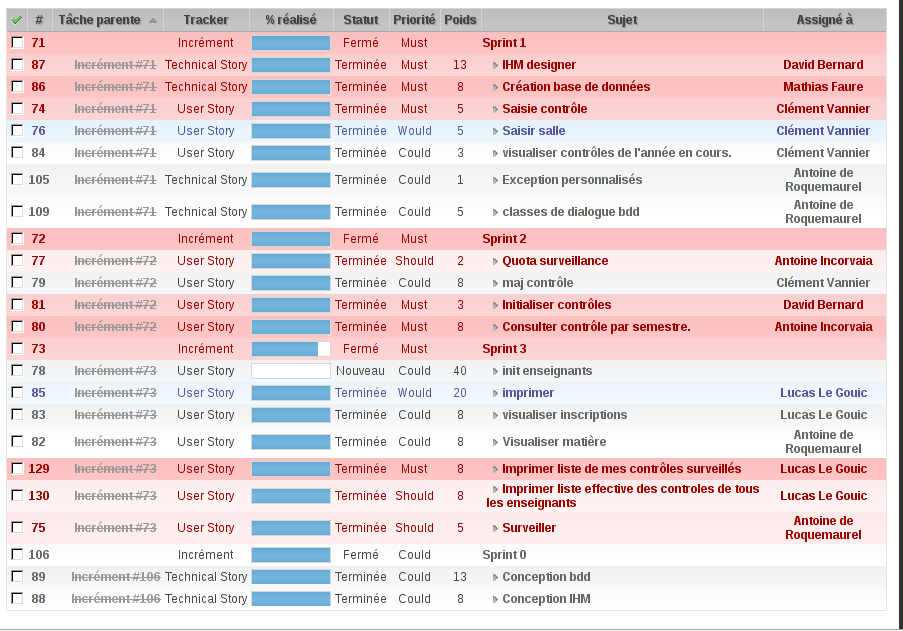
\includegraphics[width=17.5cm]{images/screenRedmine.png}
			\end{center}
			\caption{Capture d'écran des User et Technical stories dans Redmine}
		\end{figure}


\section{Planning poker}
	La technique du planning poker connait un succès grandissant auprès des équipe Scrum\footnote{En fait il ne s'agit pas de poker ni de planning, un nom plus approprié
	serait ``estimation de backlog''.}
	C'est une séance d'estimation en groupe, avec des cartes, qui combine le jugement d'expert et l'estimation par analogie.

	Ainsi, nous avons pus donner des poids aux différentes User Stories, mais nous avons également estimés les Technical stories.
	Les différents poids choisis sont disponibles en annexe \ref{tableauTaches} page \pageref{tableauTaches}.
\section{Conception}
	Une fois le planning poker effectué, nous avons effectué la conception du logiciel, étape extremement importante afin d'avoir un logiciel stable et facile à maintenir.

	Nous avons donc conçut une base de donnée qui soit facile à utilisé et qui soit la plus performante possible. 

	Nous avons également conçut l'IHM\footnote{Interface Homme Machine} du logiciel, celle-ci devauit être la plus ergonomique possible, pour avoir un logiciel facile à utiliser.

	\chapter{Sprint 1}
Au cours de ce sprint nous n'avons prévu que 3 User Stories, en effet, le sprint 1 devait être 
finit pour le 08 Mars 2012, or nous devions effectués toutes les étapes de conception 
préliminaire\footnote{cf chapitre~\ref{sprintzero}~page~\pageref{sprintzero}}.

Nous avions donc prévus d'effectuer les \USs{} suivantes:
\section{\USs{} prévues}
\subsection{Saisir contrôle}		
\begin{tabular}{ll}
	\textbf{En tant que}	&	responsable de matière\\
	\textbf{Je désire}&	saisir la date d'un contrôle, son type et sa durée\\
	\textbf{Afin de}	&	planifier les contrôles\\
	&\\
	\textbf{BVP} & Must\\
	\textbf{Poids} & 5\\
\end{tabular}
\subsection{Saisir salle}		
\begin{tabular}{ll}
	\textbf{En tant que}	&	responsable de planning\\
	\textbf{Je désire}& Renseigner une salle de surveillance\\	
	\textbf{Afin de}	& Préciser sa capacité et le nombre de surveillants nécessaires\\	
	&\\
	\textbf{BVP} & Would\\
	\textbf{Poids} & 5\\
\end{tabular}
\subsection{Visualiser contrôles de l'année en cours}
\begin{tabular}{ll}
	\textbf{En tant que}	&	Tout le monde\\
	\textbf{Je désire}&	Visualiser les contrôles de l'année universitaire en cours\\
	\textbf{Afin de}	&	\\
	&\\
	\textbf{BVP} & Could\\
	\textbf{Poids} & 3\\
\end{tabular}

\subsection{Quota surveillance} \label{usQuotaSurveillance}
Cependant nous avions mal évalués le poids des stories, ainsi, nous avons put faire la 
\story{Quota surveillance} qui été initialement prévue pour le sprint 2. 

\begin{tabular}{ll}
	\textbf{En tant que}	&	Enseignant \\
	\textbf{Je désire}&	Connaitre le nombre d'heures de surveillance effective\\
	\textbf{Afin de}	&	savoir si mon quota est atteint\\
	&\\
	\textbf{BVP} & Should\\
	\textbf{Poids} & 2\\
\end{tabular}

\section{Difficultés du sprint}
Lors de ce sprint, nous avons eu plusieurs difficultés. Principalement, la prise en main de la bibliothèque
\texttt{Qt}, mais aussi de l'EDI.
Également, le sprint zéro, avec toute la conception nous a demandés du temps, nous n'avons donc pas pus
faire beaucoup de stories. 

\section{Bilan du sprint}
À la fin du sprint, l'équipe à pus se familiariser avec les technologies utilisés. Également, nous avons
pus créer l'architecture du logiciel, étape très importante, cela nous permettra de continuer le logiciel
plus facilement et efficacement.



	\chapter{Sprint 2}
Avant le commencement de sprint, nous avons choisis de ré effectuer un planning poker,
afin de confirmer les poids des différents \USs{}.

Nous avons prévu 5 User Stories, contenant 2 must, il fallait donc faire attention, 
cependant, l'équipe s'étant habitués aux technologies, cela semblé faisable. 

Nous avons donc effectués les must sans soucis, mais nous avions sous-estimé la 
\story{surveiller}\footnote{cf section \ref{USsurveiller} page \pageref{USsurveiller}}, 
ainsi, nous n'avons pus la finir et l'avons basculé sur le sprint 3.

\section{\USs{} prévues}
\subsection{Quota surveillance}		
Cette \US{} à été effectué lors du sprint 1, cf section \ref{usQuotaSurveillance} page
\pageref{usQuotaSurveillance}.

\begin{tabular}{ll}
	\textbf{En tant que}	&	Enseignant \\
	\textbf{Je désire}&	Connaitre le nombre d'heures de surveillance effective\\
	\textbf{Afin de}	&	savoir si mon quota est atteint\\
	&\\
	\textbf{BVP} & Should\\
	\textbf{Poids} & 2\\
\end{tabular}
\subsection{Mise à jour des contrôles}		
\begin{tabular}{ll}
	\textbf{En tant que}	&	Responsable de matière\\
	\textbf{Je désire}& Modifier les informations d'un contrôle\\	
	\textbf{Afin de}	& Le mettre à jour\\	
	&\\
	\textbf{BVP} & Could\\
	\textbf{Poids} & 8\\
\end{tabular}
\subsection{Initialiser contrôles}
\begin{tabular}{ll}
	\textbf{En tant que}	&	Responsable de matière\\
	\textbf{Je désire}&	saisir en début d'année l'ensemble des contrôles\\
	\textbf{Afin de}	& planifier le contrôle continu	\\
	&\\
	\textbf{BVP} & Must\\
	\textbf{Poids} & 3\\
\end{tabular}

\subsection{Consulter contrôle par semestre}
\begin{tabular}{ll}
	\textbf{En tant que}	&	Enseignant \\
	\textbf{Je désire}&	Consulter la liste des contrôles par semestre\\
	\textbf{Afin de}	&	M'assurer de la bonne planification\\
	&\\
	\textbf{BVP} & Must\\
	\textbf{Poids} & 8\\
\end{tabular}

\subsection{Surveiller}\label{USsurveiller}
Cette \US{} n'a pus être finis durant ce sprint, en effet, nous avions sous estimé son poids, et nous
n'avons donc pas réussis à la finir avant la revue de sprint.

Nous l'avons donc basculé sur le sprint suivant.

\begin{tabular}{ll}
	\textbf{En tant que}	&	Enseignant \\
	\textbf{Je désire}&	M'ajouter à la liste des personnes d'un contrôle\\
	\textbf{Afin de}	& Surveiller\\
	&\\
	\textbf{BVP} & Should\\
	\textbf{Poids} & 5\\
\end{tabular}

\section{Difficultés du sprint}
La principale difficulté à été de ne pas avoir bien estimé le poids des \USs{}, ainsi l'équipe été
soumise à pression afin de pouvoir finir toutes les \USs{} à temps, cela n'ayant pas été possible, il 
était plus judicieux de décaler une \USs{} d'un sprint. 

Également, en cours de sprint le product owner nous à donné deux nouvelles \USs{}, nous avons donc dû les 
planifier, étant donné que nous avions déjà beaucoup de travail, nous les avons planifiés pour le 
troisième sprint.
\section{Bilan du sprint}
Ce sprint à permis d'avoir un logiciel répondant à la plupart des must exigés par le product owner.

Également, l'équipe est devenue plus soudée.


	\chapter{Sprint 3}
Avant le commencement de sprint, nous avons choisis de ré effectuer un planning poker,
afin de confirmer les poids des différents \USs{}. Nous avons donc élevé le poids 
de la \story{Surveiller}.

Nous avons prévu 7 User Stories, contenant 1 must, en effet, une \US à été basculé sur le sprint
courant\footnote{cf section \ref{USsurveiller} \pageref{USsurveiller}}, cependant elle en été à 60\%
d'avancement. 

Également, nous avions les deux nouvelles \USs{} demandés par le product owner durant le sprint 2, 
celle-ci était composé d'un Must et d'un Should, nous devions donc faire attention pour le Must.

Heureusement, 3 \US{} se ressemblait beaucoup, et était donc assez rapide à faire une fois
qu'une \US{} était effectuée, nous avions également la \story{Initialisation des enseignants} qui
avait un poids de 40, que nous avons choisis de ne pas descendre la story étant compliquée.
Celle-ci étant Could, nous nous sommes donc mis d'accord en début de sprint de d'abord effectuer les
\USs{} importantes à faire, et d'avoir un logiciel stable, étant donné que cette \USs{} aller donner
une revue de release. Si nous avions du temps, nous nous serions occupés de cette story, nous n'avons
malheureusement pas eu le temps d'effectuer cette dernière.

\section{\USs{} prévues}
\subsection{Quota surveillance}		
Cette \US{} à été effectué lors du sprint 1, cf section \ref{usQuotaSurveillance} page
\pageref{usQuotaSurveillance}.

\subsection{Surveiller}
Cette \US à été basculé sur le sprint courant étant donné que nous n'avons pus la finir précédemment. Cf
section \ref{USsurveiller}.

\begin{tabular}{ll}
	\textbf{En tant que}	&	Enseignant \\
	\textbf{Je désire}&	M'ajouter à la liste des personnes d'un contrôle\\
	\textbf{Afin de}	& Surveiller\\
	&\\
	\textbf{BVP} & Should\\
	\textbf{Poids} & 5\\
\end{tabular}

\subsection{Initialisation des enseignants}		
Cette \US{} n'a pus être effectuée par manque de temps, son poids étant important.

\begin{tabular}{ll}
	\textbf{En tant que}	&	Responsable des plannings\\
	\textbf{Je désire}& récupérer la liste des enseignants du département à partir d'un fichier Excel\textregistered\\	
	\textbf{Afin de}	& Initialiser une partie de la base de donnée\\	
	&\\
	\textbf{BVP} & Could\\
	\textbf{Poids} & 40\\
\end{tabular}
\subsection{Imprimer la liste des contrôles}
Celle-ci à un poids de 20 car cela demandera de la documentation, une fois que nous saurons imprimer
les autres \USs{} serons beaucoup plus simple, elles ont donc un poids de 8.

\begin{tabular}{ll}
	\textbf{En tant que}	&	Tout le monde \\
	\textbf{Je désire}&	imprimer la liste des contrôles de l'année universitaire en cours\\
	\textbf{Afin de}	& l'afficher\\
	&\\
	\textbf{BVP} & Would\\
	\textbf{Poids} & 20\\
\end{tabular}

\subsection{Imprimer liste de mes contrôles surveillés}
\begin{tabular}{ll}
	\textbf{En tant que}	&	Enseignant \\
	\textbf{Je désire}&	Imprimer la liste effective des contrôles surveillés avec le détail des heures\\
	&de surveillance et le cumul\\
	\textbf{Afin de}	&	pouvoir archiver à un instant donné mes surveillances\\
	&\\
	\textbf{BVP} & Must\\
	\textbf{Poids} & 8\\
\end{tabular}
\subsection{Imprimer liste effective des contrôles de tous les enseignants}
\begin{tabular}{ll}
	\textbf{En tant que}	&	Responsable de planning\\
	\textbf{Je désire}&	imprimer la liste effective des contrôles surveillés avec le détail des heures de\\
	& surveillance et de cumul de tous les enseignants triés soit par ordre alphabétique\\
	& soit par cumul croissant\\
	\textbf{Afin de}	& Archiver à un instant donné toutes les surveillances\\
	&\\
	\textbf{BVP} & Should\\
	\textbf{Poids} & 8\\
\end{tabular}



\section{Difficultés du sprint}
La difficulté du sprint était surtout le nombre de \USs{} à effectuer. Pour palier à ce problème, nous en 
avons mis une de côté, afin d'avoir un logiciel fonctionnel, avec une \US{} en moins plutôt qu'avoir
un logiciel ayant toutes les \USs{} mais ayant des bugs, ce que le product owner ne souhaite surtout pas.

\section{Bilan du sprint}
Nous avons donc pus effectuer toutes les \US{} que nous voulions au début du sprint. L'impression qui
pouvait poser des problème n'a posé aucun problème, celui-ci étant de se documenter, nous avons pus
trouver comment imprimer. 

À la fin de ce sprint, nous avons effectués une revue de release qui s'est passé sans encombre.


	\include{includes/synthese}
	\appendix
	\chapter{Les différentes tâches}\label{tableauTaches}
Page suivante, vous pourrez obtenir le récapitulatif de toutes les tâches, User stories et Technical stories qui ont été effectués pour mener à bien ce projet.
Chaque tâche à été assignée à une personne du groupe, vous pouvez également voir le pourcentage effectués des tâches. Le pdf ayant été généré a la fin du projet
celles-ci sont toutes à 100\% sauf les stories n'ayant pus être faite.
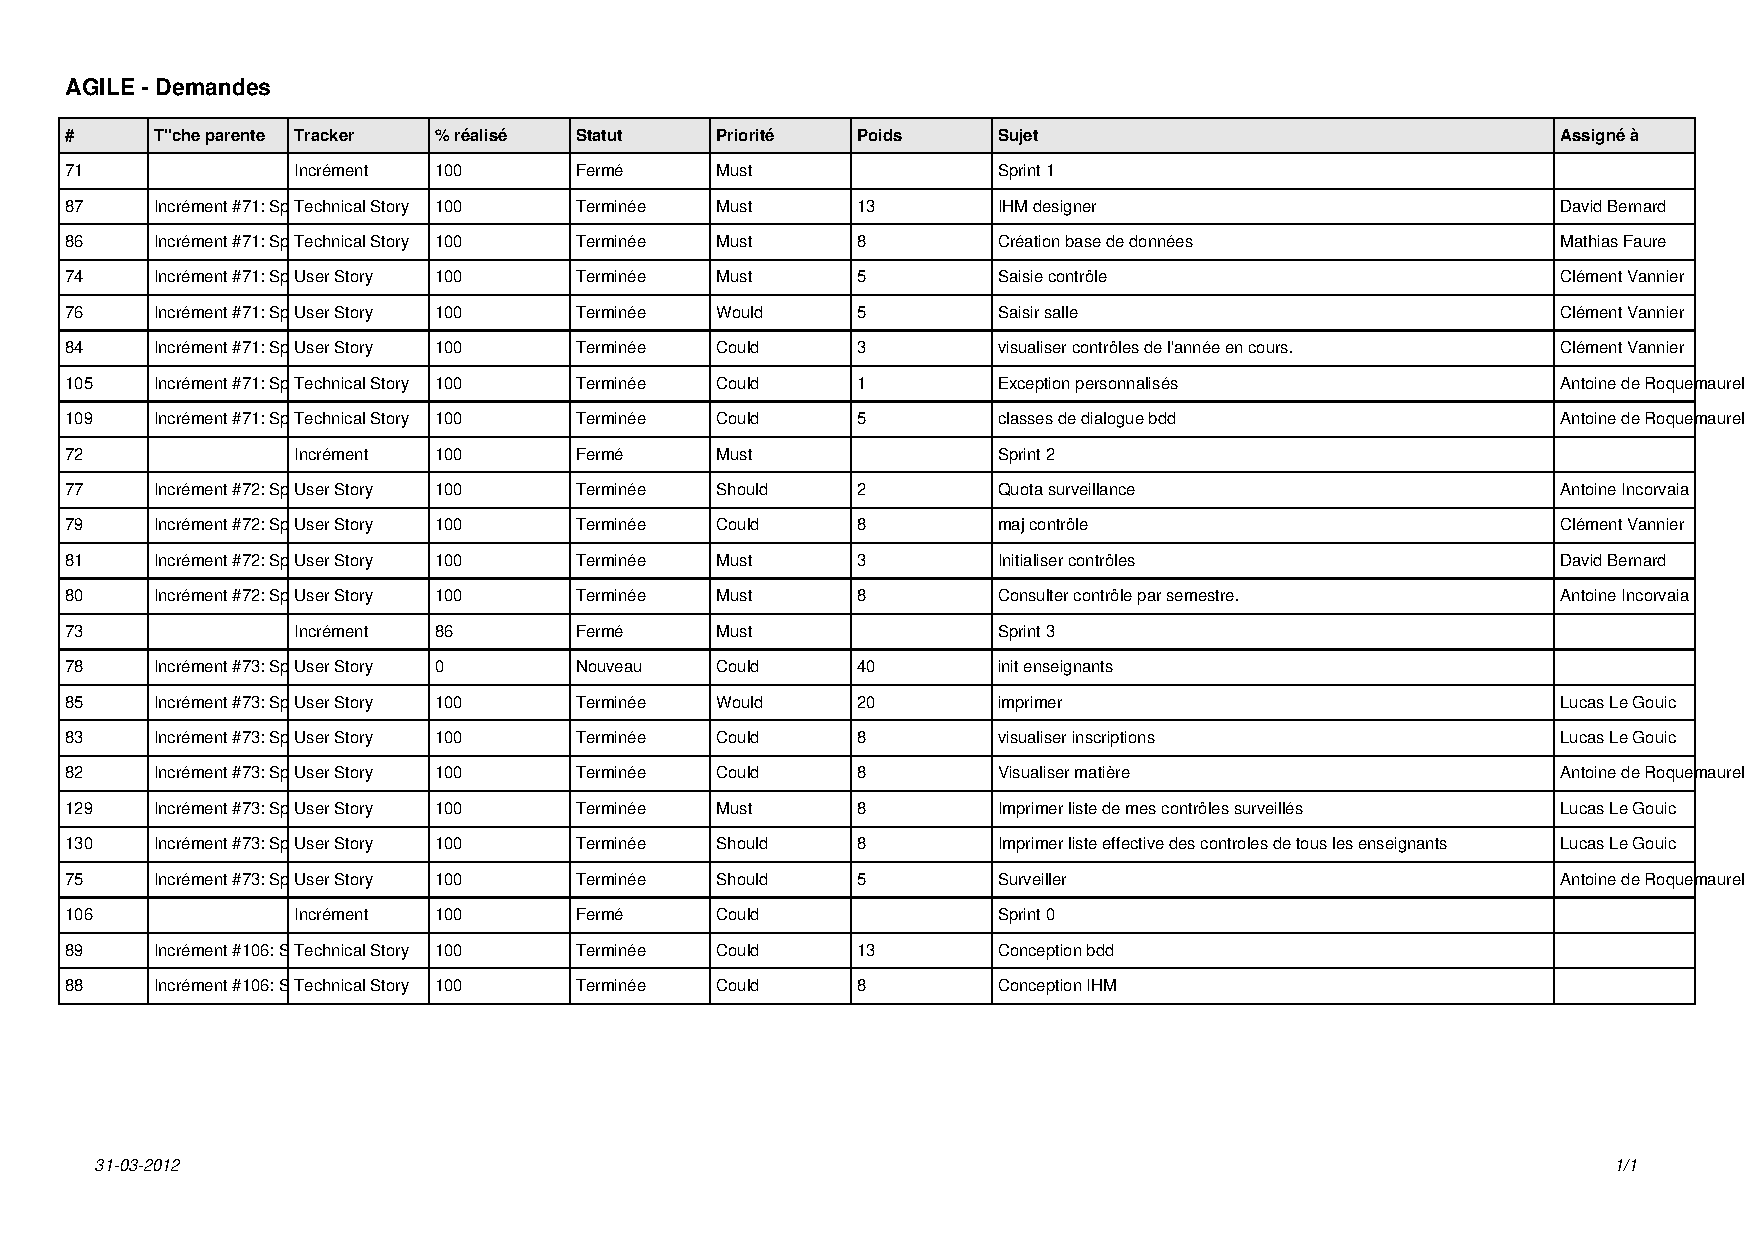
\includepdf[landscape]{images/tachesRedmine.pdf}


\end{document}






